\section{性能分析及系统展示}
\label{sec:experiment}

\subsection{围绕目标的端到端性能分析}

本作品的性能验证围绕赛题一评分要求和真实风控目标展开，重点证明系统同时具备实时性、准确性、可解释性和溯源性，而不是只报告单一分类指标。实验覆盖离线主模型、实时链路、API延迟、阈值策略、团伙挖掘、GraphSAGE旁路以及部署清单结构验证。

\begin{table}[H]
  \centering
  \caption{实验验证项目}
  \label{tab:experiment_items}
  \renewcommand\arraystretch{1.35}
  \setlength{\tabcolsep}{5pt}
  {\songti\zihao{5}
  \begin{tabularx}{0.96\textwidth}{>{\raggedright\arraybackslash}p{2.2cm}>{\raggedright\arraybackslash}X>{\raggedright\arraybackslash}X}
    \toprule
    实验类别 & 验证目标 & 对应脚本或接口 \\
    \midrule
    离线训练评估 & 比较模型PR-AUC、ROC-AUC、F1、Top 1\%召回和误报率 & \code{python -m fraudsim.training.train} \\
    实时链路验证 & 验证Kafka输入、Flink评分、告警输出和迟到事件输出 & \code{producer}、\code{flink\_job.py}、\code{/topics/\{topic\}/recent} \\
    API延迟压测 & 比较单笔评分与批量评分的平均、P50、P95、P99延迟 & \code{scripts/benchmark\_api\_latency.py} \\
    图挖掘验证 & 验证疑似团伙、共享资源证据、实体风险特征是否生成 & \code{python -m fraudsim.graph\_mining} \\
    阈值与图学习 & 验证业务阈值影响和GraphSAGE图嵌入价值 & \code{/threshold-sandbox}、\code{graphsage\_experiment} \\
    部署与安全 & 验证K8s资源结构、敏感接口认证和审计链路 & K8s单元测试、\code{/audit/recent} \\
    \bottomrule
  \end{tabularx}
  }
\end{table}

\subsubsection{准确性：离线模型与业务阈值}

训练脚本使用训练集拟合模型、验证集校准阈值、测试集报告最终指标。输出指标包括PR-AUC、ROC-AUC、F1、Top 1\%召回率和高风险阈值下误报率。其中PR-AUC适合衡量欺诈样本稀少情况下的排序质量；Top 1\%召回率模拟风控团队有限审核资源下的重点拦截能力；误报率反映正常用户体验损失。

推荐复现实验命令如下：

\begin{lstlisting}[language=bash]
python -m fraudsim.training.train --dataset fp_fraudsim_injected --model lightgbm
python -m fraudsim.training.train --dataset fp_fraudsim_injected --model xgboost
python -m fraudsim.training.train --dataset fp_fraudsim_injected --model catboost
python -m fraudsim.training.train --dataset fp_fraudsim_injected --model sklearn_hgb
\end{lstlisting}

已记录的LightGBM主模型实验使用67个特征，在123,649条测试交易上取得PR-AUC 0.9727、ROC-AUC 0.9949、F1 0.9169，高风险阈值下误报率为0.338\%。模型训练后，\code{models/leaderboard.json}按PR-AUC排序。当前代码仓库未包含大体积数据和模型产物，复现时需按README完成数据准备与训练，并以重新生成的\code{metrics.json}核验结果。

\begin{figure}[H]
  \centering
  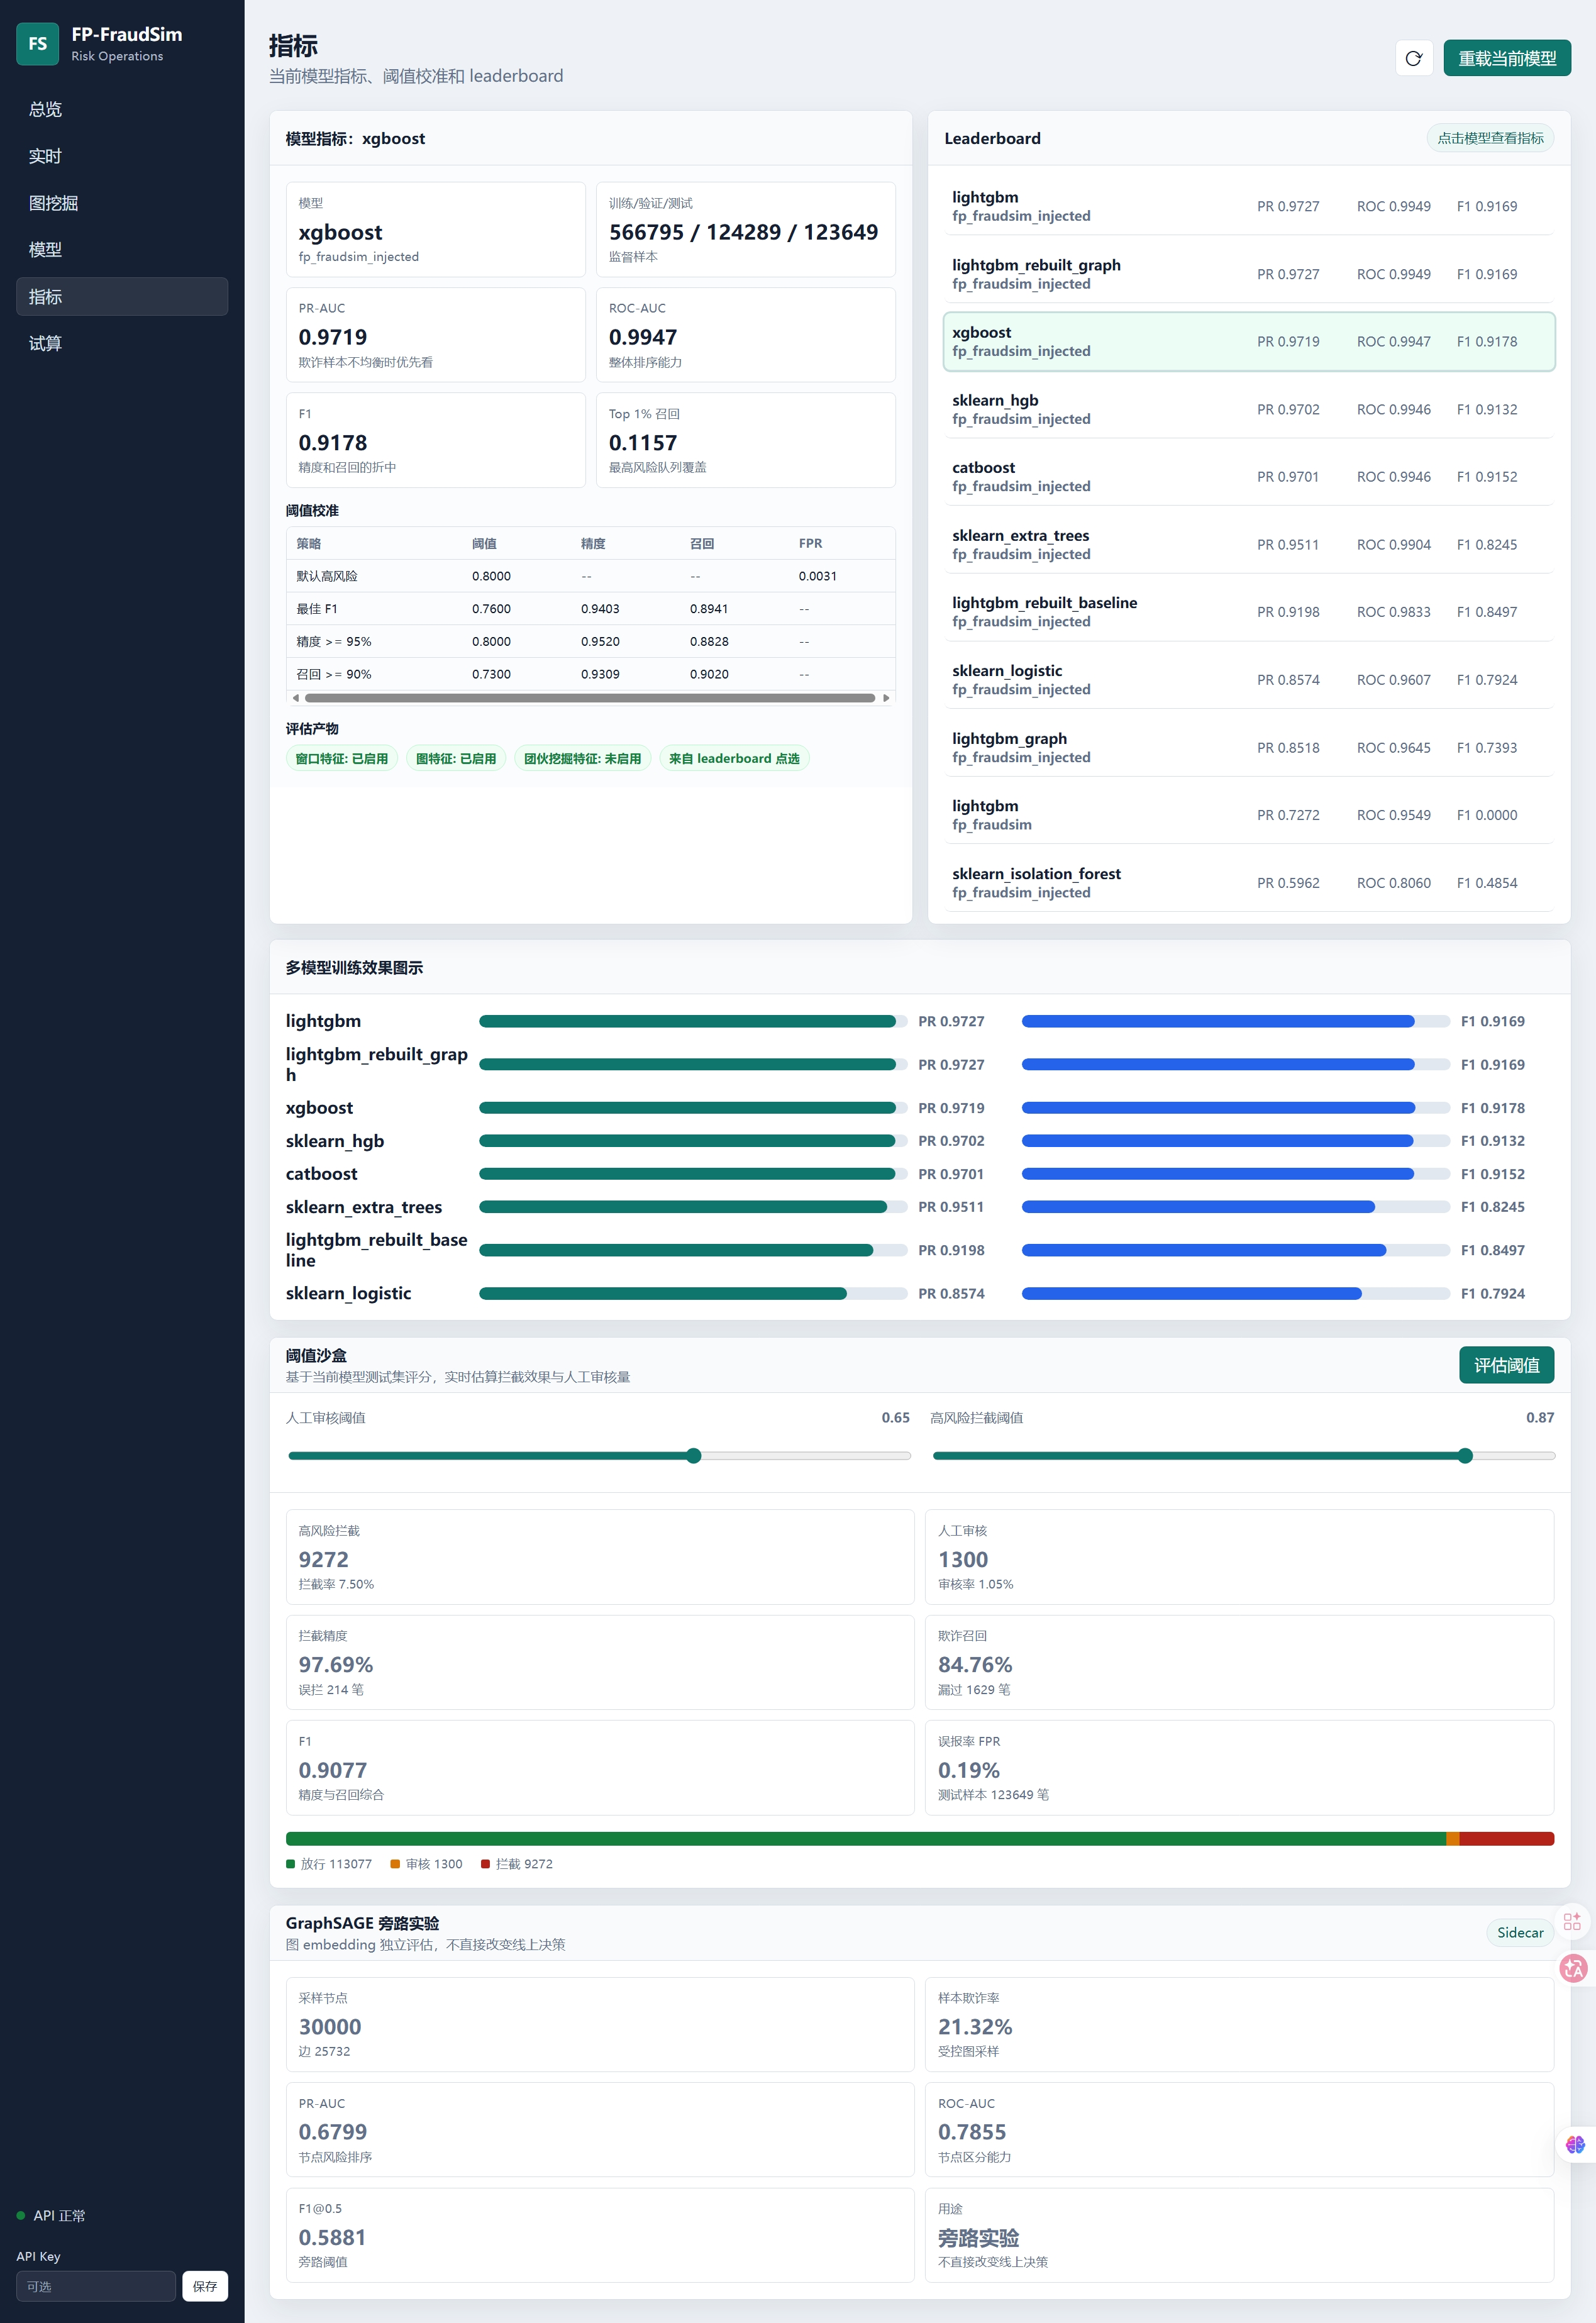
\includegraphics[width=0.68\textwidth]{pic/dashboard_model_metrics_report.png}
  \caption{多模型指标对比、排行榜与阈值评估界面}
  \label{fig:dashboard_model_metrics}
\end{figure}

\subsubsection{实时性：端到端链路与接口延迟}

系统提供Docker Compose一键部署。推荐流程为先训练模型，再启动Kafka、Redis、Model API和Flink风险作业，随后创建主题、加载画像并回放交易流。

\begin{lstlisting}[language=bash]
docker compose -p fraudsim up -d --build kafka redis model-api flink-jobmanager flink-taskmanager flink-risk-job
python -m fraudsim.streaming.topics --bootstrap-servers localhost:9094
python -m fraudsim.streaming.load_profiles --dataset fp_fraudsim_injected --redis-url redis://localhost:6379/0
python -m fraudsim.streaming.producer --dataset fp_fraudsim_injected --bootstrap-servers localhost:9094 --rate 100 --limit 1000
\end{lstlisting}

风险结果可通过Dashboard查看，也可通过API读取Kafka近期消息。实时输出字段包括\code{transaction\_id}、\code{risk\_score}、\code{risk\_level}、\code{decision}、\code{reason\_codes}、模型名称、模型版本和评分时间。该输出满足赛题要求的“风险评估、欺诈判定和风险等级输出”。

\subsubsection{接口压测与微批吞吐优化}

API延迟压测脚本先调用\code{/health}确认模型已加载，再分别测试单笔和批量\code{/predict}。本机Docker Compose实测中，单笔请求平均延迟115.78毫秒，P95为156.55毫秒，P99为240.30毫秒；每批25条时，批量请求平均耗时125.00毫秒，平均单条折算为5.00毫秒，P95折算为6.16毫秒，平均单条吞吐收益为23.16倍。

\begin{lstlisting}[language=bash]
python scripts/benchmark_api_latency.py --api-url http://localhost:8000 --records 200 --batch-size 50
\end{lstlisting}

在线流式作业默认批大小50、最长等待300毫秒，并使用flush marker主动刷新尾批。完整链路已验证Flink作业处于RUNNING状态、100条交易成功回放，\code{risk\_results}能够输出窗口、画像、图风险、决策和理由码。

\subsubsection{可解释性与溯源性：阈值和图分析}

阈值沙盒在\code{medium=0.50}、\code{high=0.80}时记录到放行112,249条、人工审核1,647条、高风险拦截9,753条，拦截精度96.08\%、欺诈召回87.69\%、误报率0.338\%。该实验说明阈值应结合误报成本和审核容量配置，而不能只以模型F1最大化为目标。

\begin{figure}[H]
  \centering
  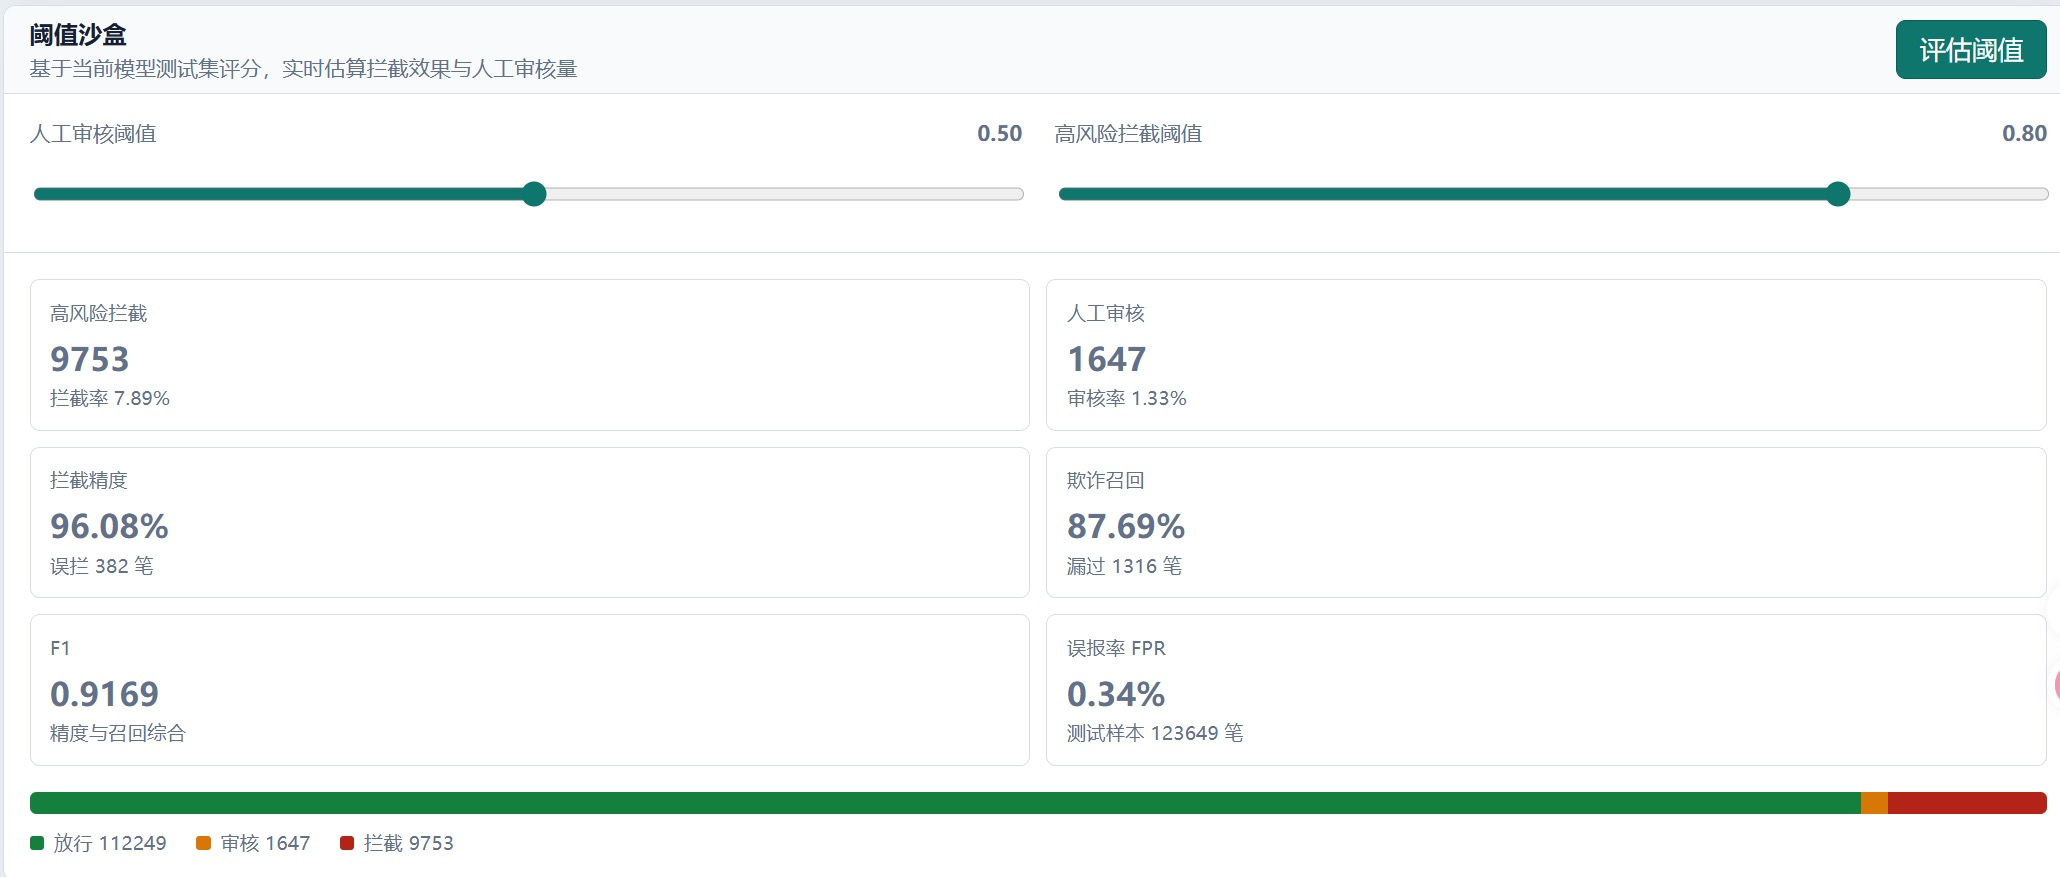
\includegraphics[width=0.96\textwidth]{pic/dashboard_threshold_report.png}
  \caption{阈值沙盒中的拦截效果与人工审核量评估}
  \label{fig:dashboard_threshold}
\end{figure}

可解释图挖掘记录到475个候选团伙；在0.65高置信阈值下，交易精度为98.71\%，注入团伙总体召回为77.93\%。GraphSAGE旁路实验采样30,000个节点和25,732条边，取得PR-AUC 0.6799、ROC-AUC 0.7855和F1@0.5为0.5881。结果证明图嵌入具有识别价值，但当前效果和时序验证尚不足以替代线上主模型，因此保持旁路。

\subsection{消融实验分析}

消融实验用于回答不同算法、参数和模块是否真正改善系统目标。表~\ref{tab:ablation_analysis}汇总当前已完成的受控对比。结果表明：微批评分显著降低单条折算耗时；图挖掘能够补充交易级模型无法直接给出的团伙证据；GraphSAGE具备研究价值，但当前指标不足以替代主模型；双阈值策略能够将模型分数转化为可控的审核工作量。

\begin{table}[H]
  \centering
  \caption{关键算法、参数与模块消融分析}
  \label{tab:ablation_analysis}
  \renewcommand\arraystretch{1.32}
  \setlength{\tabcolsep}{4pt}
  {\songti\zihao{5}
  \begin{tabularx}{0.98\textwidth}{>{\raggedright\arraybackslash}p{2.4cm}>{\raggedright\arraybackslash}p{3.0cm}>{\raggedright\arraybackslash}X>{\raggedright\arraybackslash}p{3.0cm}}
    \toprule
    对比项 & 基线/消融设置 & 关键结果 & 结论 \\
    \midrule
    单笔与微批推理 & 单笔请求；25条/批 & 单笔平均115.78ms；微批单条折算5.00ms，收益23.16倍 & 微批是高并发实时链路的关键优化 \\
    交易模型与图旁路 & LightGBM主模型；GraphSAGE旁路 & 主模型PR-AUC 0.9727；图旁路PR-AUC 0.6799 & 图嵌入暂不替代稳定主模型 \\
    无图解释与图挖掘 & 仅风险分数；增加共享资源与连通分量 & 发现475个候选团伙，高置信交易精度98.71\% & 图模块显著增强解释与溯源能力 \\
    单阈值与双阈值 & 直接二分类；$T_1=0.50,T_2=0.80$ & 形成放行112,249、复核1,647、拦截9,753的可控分流 & 双阈值连接准确率与审核容量 \\
    固定输入与可调仿真 & 固定增强集；调整欺诈率、团伙规模和速率 & 可生成不同难度和负载的复现实验流 & 增强稳定性与压力测试覆盖 \\
    \bottomrule
  \end{tabularx}}
\end{table}

\subsection{系统界面截图与任务自评}

表~\ref{tab:task_self_assessment}按照赛题一必须完成的任务进行形式检查和自评估，并给出可直接核验的界面或工程证据。自评结果用于定位交付完整性，不替代评委最终评分。

\begin{table}[H]
  \centering
  \caption{赛题一任务形式检查与自评估}
  \label{tab:task_self_assessment}
  \renewcommand\arraystretch{1.28}
  \setlength{\tabcolsep}{3.5pt}
  {\songti\zihao{5}
  \begin{tabularx}{0.98\textwidth}{>{\raggedright\arraybackslash}p{2.5cm}>{\centering\arraybackslash}p{1.2cm}>{\raggedright\arraybackslash}X>{\raggedright\arraybackslash}p{3.2cm}}
    \toprule
    必须任务 & 状态 & 核验内容 & 对应证据 \\
    \midrule
    仿真环境与实时检测 & 已完成 & 七类场景、可调仿真、交易回放与实时风险分级 & 仿真脚本、总览、回放与告警界面 \\
    流式数据处理框架 & 已完成 & Kafka、Flink事件时间、watermark、窗口与迟到分流 & Compose、Flink作业、风险主题 \\
    自适应学习与迭代 & 已完成 & 反馈样本池、Candidate、Latest、Rollback与热切换 & 回放反馈页、模型指标页、接口 \\
    多维度特征构建 & 已完成 & 交易、画像、窗口、设备/IP、商户和图关联特征 & 特征表、理由码页、图团伙页 \\
    性能测试与解释溯源 & 已完成 & 延迟、准确率、阈值、理由码、团伙证据链 & 性能表、阈值页、团伙网络页 \\
    安全与工程交付 & 已完成 & API Key、审计、部署隔离、测试与复现文档 & 安全方案、K8s清单、附录清单 \\
    \bottomrule
  \end{tabularx}}
\end{table}

\begin{figure}[H]
  \centering
  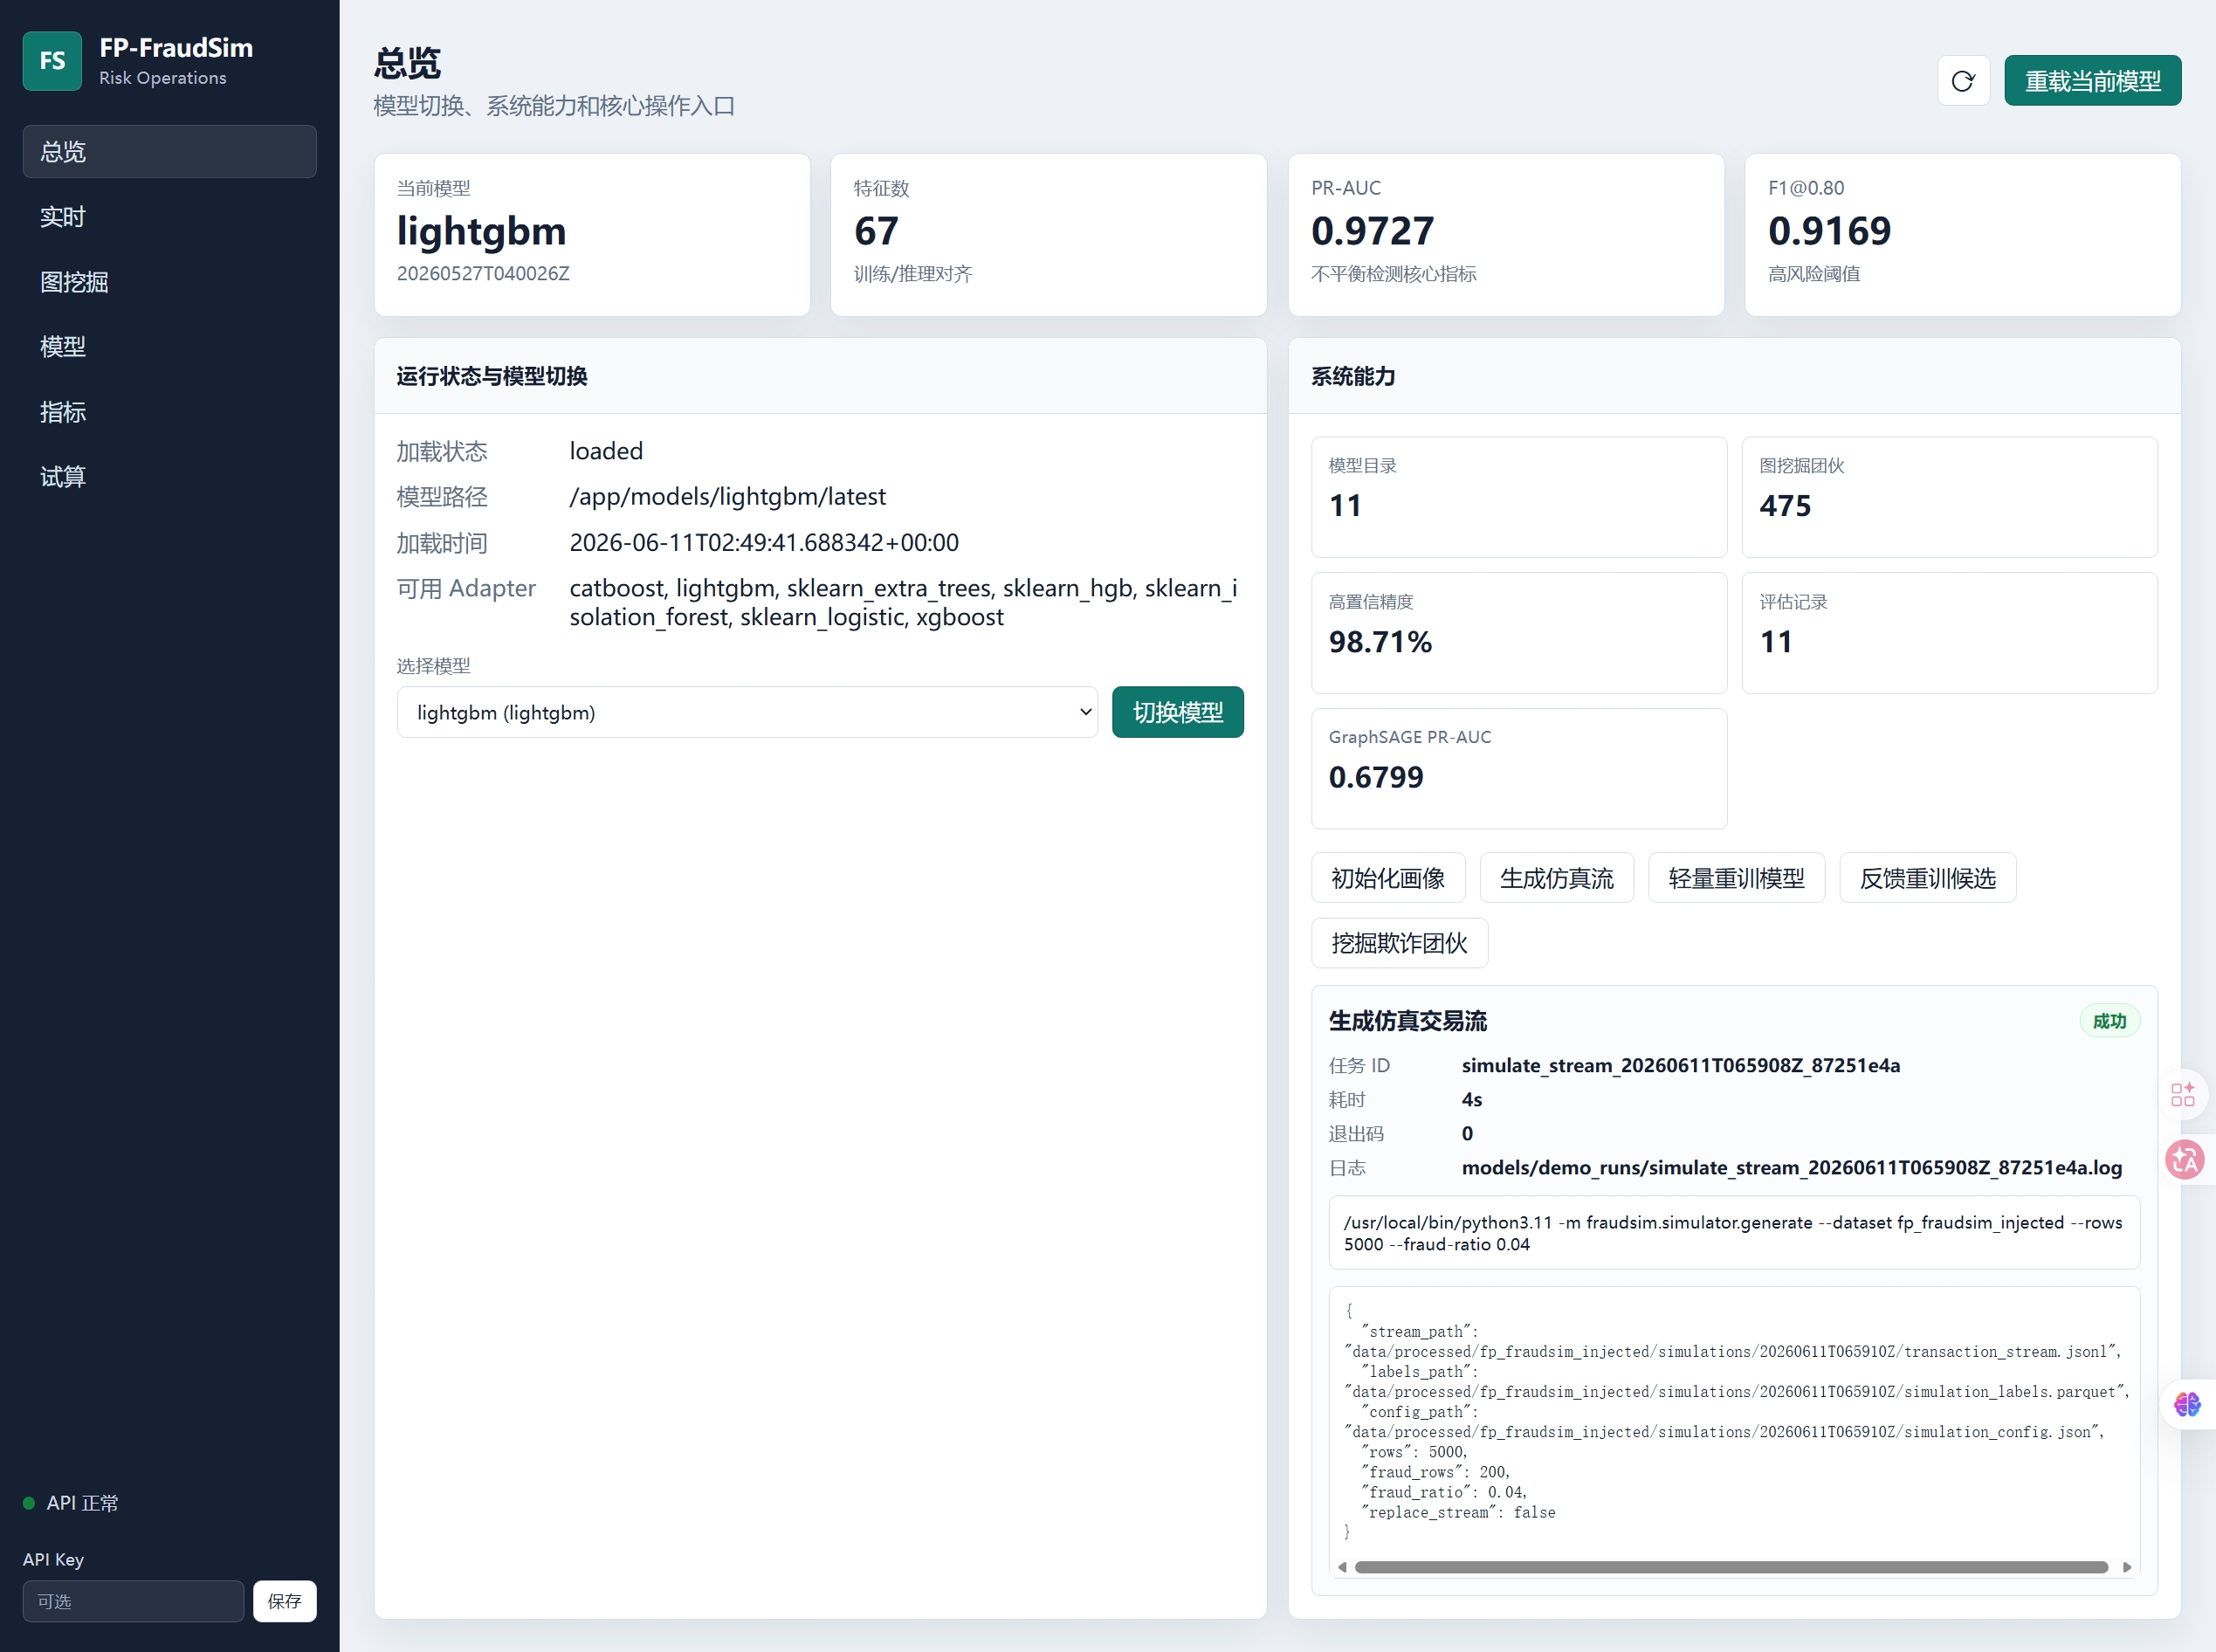
\includegraphics[width=0.92\textwidth]{pic/dashboard_overview_report.png}
  \caption{系统总览、服务状态与实时任务入口}
\end{figure}

\begin{figure}[H]
  \centering
  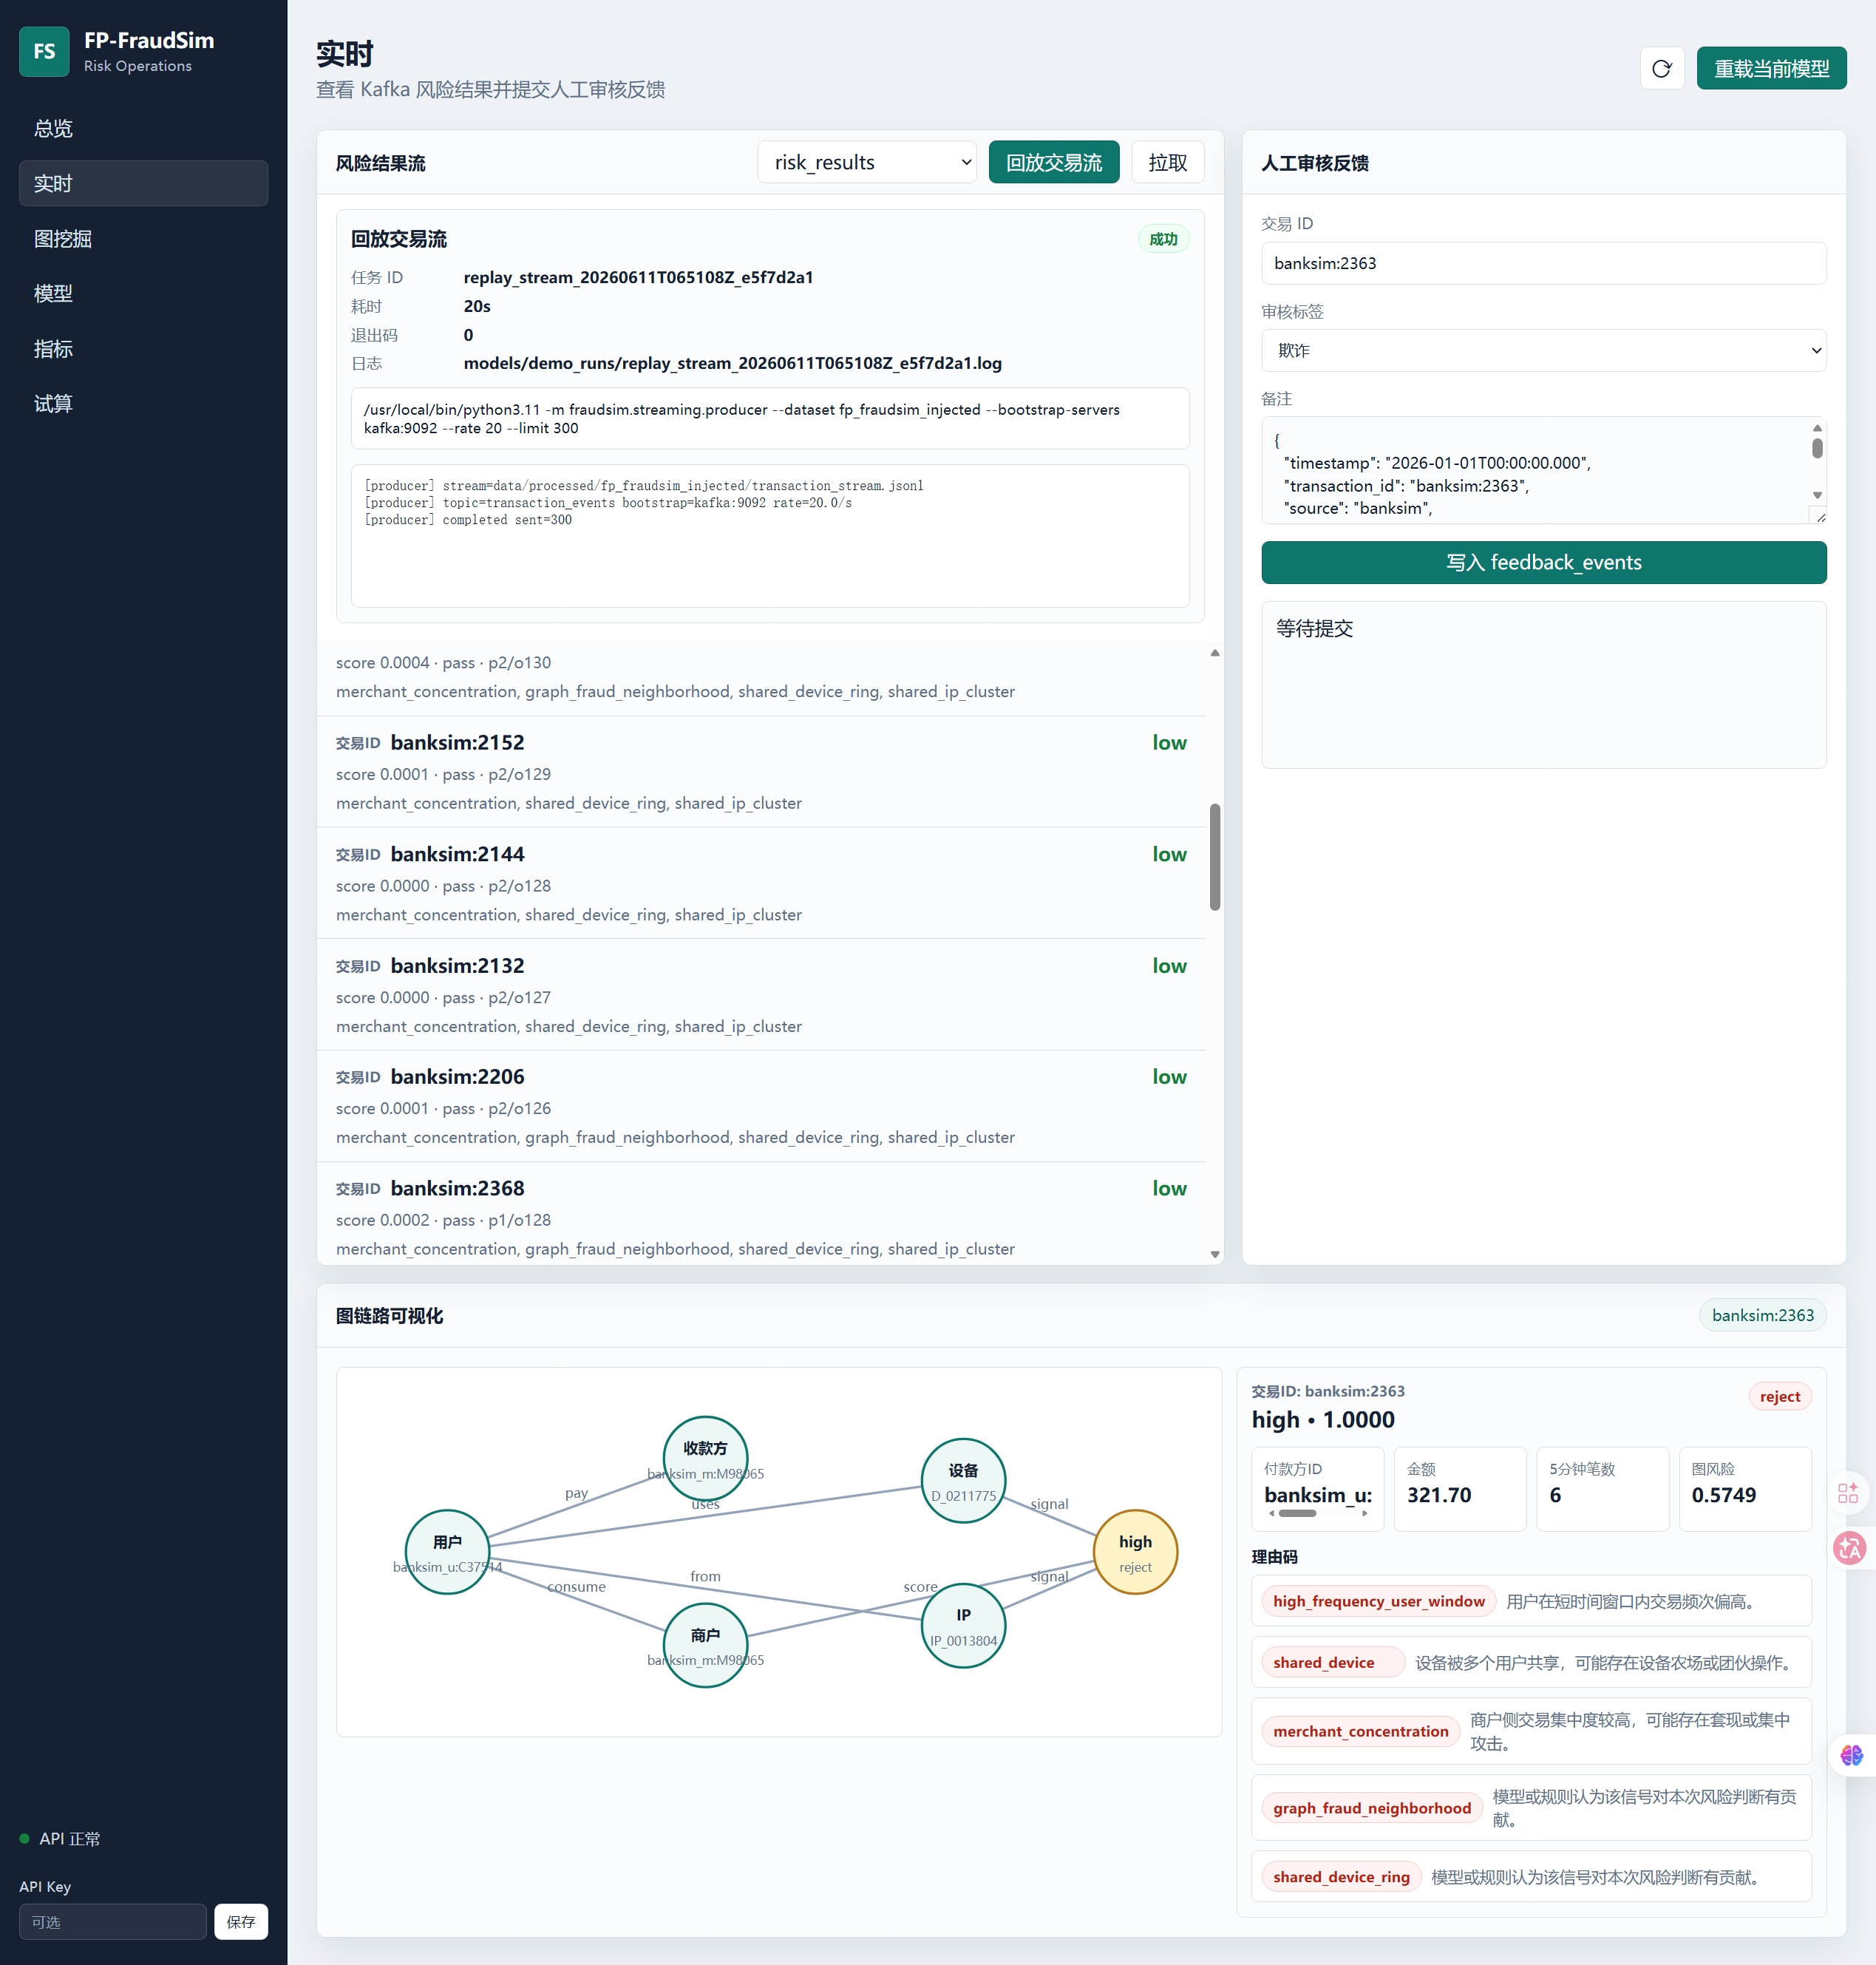
\includegraphics[width=0.82\textwidth]{pic/dashboard_replay_feedback_report.png}
  \caption{交易回放、风险结果与人工反馈闭环}
\end{figure}

\subsection{交付清单与复现保障}

项目交付包括代码工程、部署文件、测试、技术文档、指标报告和Dashboard。详细逐项交付清单见附录C；核心自动化测试覆盖如下。

\subsubsection{自动化测试覆盖}

项目包含面向核心模块的单元测试，除原有特征、窗口、微批、图挖掘和API测试外，新增可调仿真器、阈值沙盒、GraphSAGE数据构建和Kubernetes清单结构测试。

\begin{itemize}
  \item \code{test\_features.py}：验证训练特征选择、缺失填充和类别处理；
  \item \code{test\_window\_features.py}：验证用户、设备、IP、商户窗口统计；
  \item \code{test\_streaming\_microbatch.py}：验证微批评分缓冲与flush逻辑；
  \item \code{test\_graph\_mining\_explainability.py}：验证团伙挖掘和解释字段；
  \item \code{test\_api\_dashboard.py}：验证Dashboard资源、模型发现、指标和模型重载。
  \item \code{test\_simulator.py}与\code{test\_threshold\_sandbox.py}：验证仿真配置和阈值指标计算；
  \item \code{test\_graphsage\_experiment.py}与\code{test\_k8s\_manifests.py}：验证图采样、节点标签和边云资源清单。
\end{itemize}

测试运行命令为：

\begin{lstlisting}[language=bash]
python -m unittest discover -s tests
\end{lstlisting}
